%&pdflatex
%% filename: amsart-template.tex, version: 2.1
\documentclass[reqno]{amsart}

\usepackage{hyperref}
\usepackage{inputenc}
\usepackage{graphicx}
\usepackage{bbm}
\usepackage{amssymb}
\usepackage{listings}
\usepackage{float}



\newtheorem{theorem}{Theorem}[section]
\newtheorem{lemma}[theorem]{Lemma}
\theoremstyle{definition}
\newtheorem{definition}[theorem]{Definition}
\newtheorem{example}[theorem]{Example}
\newtheorem{xca}[theorem]{Exercise}
\theoremstyle{remark}
\newtheorem{remark}[theorem]{Remark}
\numberwithin{equation}{section}
\setlength{\parindent}{0pt} % turn off auto-indent

\graphicspath{ {./} }

\begin{document}

\title{Assignment 3: [IFT6390]}

\author{L\'ea Ricard \& Joseph D. Viviano}
\address{Universit\'e de Montr\'eal}
\curraddr{}
\email{joseph@viviano.ca, lea.ricard@umontreal.ca}
\thanks{}
\date{Oct 2018}

\maketitle
%------------------------------------------------------------------------------
%--------------------Theorical part a--------------
%------------------------------------------------------------------------------
\section{Derivatives and relationships between basic functions}

%1.1
\subsection{}
\begin{align}
    sigmoid(x) &= \frac{1}{2} \Bigg( tanh(\frac{1}{2}x) + 1 \Bigg) \\
    &= \frac{1}{2} \Bigg(\frac{ e^{\frac{1}{2}x} - e^{\frac{-1}{2}x}}{ e^{\frac{1}{2}x} + e^{\frac{-1}{2}x} } + 1 \Bigg) \\
\end{align} \\

We substitue 1 for $\frac{ e^{\frac{1}{2}x} + e^{\frac{-1}{2}x}}{ e^{\frac{1}{2}x} + e^{\frac{-1}{2}x} }$ to get: \\

\begin{align}
    sigmoid(x) &= \frac{1}{2} \Bigg(\frac{ e^{\frac{1}{2}x} - e^{\frac{-1}{2}x}}{ e^{\frac{1}{2}x} + e^{\frac{-1}{2}x} } + 
                                    \frac{ e^{\frac{1}{2}x} + e^{\frac{-1}{2}x}}{ e^{\frac{1}{2}x} + e^{\frac{-1}{2}x} } \Bigg) \\
               &= \frac{1}{2} \Bigg(\frac{ e^{\frac{1}{2}x} - e^{\frac{-1}{2}x} + e^{\frac{1}{2}x} + e^{\frac{-1}{2}x} }{ e^{\frac{1}{2}x} + e^{\frac{-1}{2}x} } \Bigg) \\
               &= \frac{1}{2} \Bigg(\frac{ e^{\frac{1}{2}x} + e^{\frac{1}{2}x} }{ e^{\frac{1}{2}x} + e^{\frac{-1}{2}x} } \Bigg) \\
               &= \frac{1}{2} \Bigg(\frac{ 2 e^{\frac{1}{2}x} }{ e^{\frac{1}{2}x} + e^{\frac{-1}{2}x} } \Bigg) \\
               &= \frac{ 1 }{ 1 + e^{-x} }
\end{align}

%1.2
\subsection{}
\begin{align}
    ln(sigmoid(x)) &= ln(\frac{1}{1 + e^{-x}}) \\
    &= ln(1) - ln(1 + e^{-x}) \\
    &= -ln(1 + e^{-x}) \\
    &= -softmax(-x)
\end{align}

%1.3
\subsection{}
\begin{align}
    \frac{dsigmoid}{dx}(x) &= \frac{d}{dx}(\frac{1}{1+e^{-x}}) \\
    &= \frac{d}{dx} (1 - e^{-x})^{-1} \\
    &= [-1][1 + e^{-x}]^{-2} \frac{d}{dx}[1 + e^{-x}] \\
    &= [-1][1 + e^{-x}]^{-2} [e^{-x}] \frac{d}{dx}[-x]\\
    &= [-1][1 + e^{-x}]^{-2} [e^{-x}] [-1] \\
    &= \frac{e^{-x}}{(1+ e^{-x})^{2}}
\end{align}

We can rewrite the last result as:

\begin{align}
    \frac{e^{-x}}{(1+ e^{-x})^{2}} &= \frac{e^{-x} +1 -1}{(1 + e^{-x})^2} \\
    &= \frac{1 + e^{-x}}{(1 + e^{-x})^2} - \frac{1}{(1 + e^{-x})^2} \\
    &= \frac{1}{1 + e^{-x}}  - \frac{1}{(1 + e^{-x})^2}\\
    &= \frac{1}{1 + e^{-x}} - \frac{1}{(1 + e^{-x})}\frac{1}{(1 + e^{-x})}\\
    &= \frac{1}{1 + e^{-x}} (1- \frac{1}{1 + e^{-x}})\\
    &= sigmoid(x)(1 - sigmoid(x))
\end{align}

%1.4
\subsection{}

\begin{align}
    \frac{dtanh}{dx}(x) &= \frac{d}{dx}(\frac{e^x-e^{-x}}{e^x+e^{-x}}) \\
    &= \frac{\frac{d}{dx}(e^x-e^{-x})(e^x+e^{-x}) -  \frac{d}{dx}(e^x+e^{-x})(e^x-e^{-x})}{(e^x+e^{-x})^2} \\
    &= \frac{(e^x+e^{-x})(e^x+e^{-x}) - (e^x-e^{-x})(e^x-e^{-x})}{(e^x+e^{-x})^2}\\
    &= \frac{(e^x+e^{-x})^2}{(e^x+e^{-x})^2} - \frac{(e^x-e^{-x})^2}{(e^x+e^{-x})^2}\\
    &= 1- tanh^2(x)
\end{align}

%1.5
\subsection{}

\begin{align}
    sign(x) &\coloneqq \begin{cases}
        1 & x > 0 \\
        0 & x = 0 \\
        -1 & x < 0
    \end{cases}
\end{align}

Can be written as athe sum of two indicator functions: \\

\begin{align}
    sign(x) = \textbf{1}_{\{x > 0\}} - \textbf{1}_{\{x < 0\}}
\end{align}\\

$x = 0$ is handled implicitly by this notation, because it matches neither condition.


%1.6
\subsection{}

\begin{align}
    abs'(x) = sign(x) = \frac{ \partial }{ \partial x } |x| = \textbf{1}_{\{x > 0\}} - \textbf{1}_{\{x < 0\}}
\end{align}

Where $abs'(x)$ is technically undefined at zero, but is simply set to 0 using the above notation.

%1.7
\subsection{}

The rectifier function is 0 for all $x \leq 0$, so:

\begin{align}
    rect'(x) = \textbf{1}_{\{x > 0\}} 
\end{align}

%1.8
\newcommand\norm[1]{\left\lVert#1\right\rVert}

\subsection{}

If $\norm{x}^2_{2} = \sum_{i} x_i^2$, then the gradient is: \\

\begin{align}
    \frac{\partial \norm{x}^2_{2}}{\partial x} &= \frac{\partial}{\partial x} \sum_i x_i^2 \\
    &= \sum_i \frac{\partial}{\partial x} x_i^2 \\
    &= \sum_i 2x_i
\end{align}

%1.9
\subsection{}

If $\norm{x}_{1} = \sum_{i} |x_i|$, then the gradient is: \\

\begin{align}
    \frac{\partial \norm{x}_{1}}{\partial x} &= \frac{\partial}{\partial x} \sum_i |x_i| \\
    &= \sum_i \frac{\partial}{\partial x} |x_i| \\
    &= \sum_i sign(x_i) \\
    &= \sum_i \textbf{1}_{\{x > 0\}} - \textbf{1}_{\{x < 0\}}
\end{align}\\

%------------------------------------------------------------------------------
%--------------------Theorical part b--------------
%------------------------------------------------------------------------------
\section{Gradient computation for parameters optimization in a neural net for multiclass classification}

%2.1
\subsection{}

The dimension of $\mathbf{b}^{(1)}$ is: $\mathbf{b^{(1)}} \in \mathbb{R}^{d_h}$. \\

\begin{equation}
    \mathbf{h}^a = \mathbf{W}^{(1)T} \cdot \mathbf{x} + \mathbf{b}^{(1)}
\end{equation}

\begin{equation}
    \mathbf{h}_j^a = \mathbf{W}_j^{(1)T} \cdot \mathbf{x} + b_j^{(1)}
\end{equation}

\begin{equation}
    \mathbf{h}^s = g(\mathbf{h}^a)
\end{equation}

Where $g(x)$ is the activation function (i.e., ReLU nonlinearity) applied element wise to the hidden layer. $g(x) = max(0,x)$.

%2.2
\subsection{}
The dimensions of $\mathbf{W}^{(2)}$ and $\mathbf{b}^{(2)}$ are:
$\mathbf{W}^{(2)} \in \mathbb{R}^{m \times d_h}$, and $\mathbf{b}^{(2)} \in \mathbb{R}^{m}$. \\

\begin{equation}
    \mathbf{o}^a = \mathbf{W}^{(2)T} \cdot \mathbf{h^s}+ \mathbf{b}^{(2)}
\end{equation}

\begin{equation}
    \mathbf{o}_k^a = \mathbf{W}_k^{(2)T} \cdot \mathbf{h^s}+ b_k^{(2)}
\end{equation}

%2.3
\subsection{}

Let's define an m-class softmax: $softmax(x) = \frac{e^{x_i}}{\sum_{i=1}^m e^{x_i}}$. Therefore, \\

\begin{equation}
    \mathbf{o}_k^s = \frac{e^{\mathbf{o}_k^a}}{\sum_{i=1}^m e^{\mathbf{o}_k^a}}
\end{equation}

\begin{align}
\sum_{i=1}^m \mathbf{o}_k^s 
&= \sum_{i=1}^m \frac{e^{\mathbf{o}_k^a}}{\sum_{i=1}^m e^{\mathbf{o}_k^a}} \\
&= \frac{\sum_{i=1}^m e^{\mathbf{o}_k^a}}{\sum_{i=1}^m e^{\mathbf{o}_k^a}} \\
&= 1.
\end{align}

Since $e^x > 0$, the result will always be positive. This is crucial because we need the softmax to produce a probability  distribution over our $m$ output classes.

%2.4
\subsection{}

\begin{equation}
L(\mathbf{o}^a, y) = -\sum_{k=1}^M y_{k}\log \Bigg(     
    \frac{e^{\mathbf{o}_k^a}}{\sum_{i=1}^m e^{\mathbf{o}_k^a}}
\Bigg)
\end{equation}


%2.5
\subsection{}
The set of parameters is:

\begin{equation}
    \theta = \{\mathbf{W}^{(1)},\mathbf{b}^{(1)}, \mathbf{W}^{(2)}, \mathbf{W}^{(2)}\}
\end{equation}

Since $\mathbf{W}^{(1)} \in \mathbb{R}^{d_h \times d}$, $\mathbf{b}^{(1)} \in \mathbb{R}^{d_h}$, $\mathbf{W}^{(2)} \in \mathbb{R}^{m \times d_h}$, and $\mathbf{b}^{(2)} \in \mathbb{R}^{m}$, there is a total of $n_\theta= d_h \times (d+1) + m \times (d_h+1)$ scalar parameters.\\

The empirical risk $\hat{R}$ associated with the lost function is:

\begin{equation}
    \hat{R} = \frac{1}{n}\sum_{i=1}^{n} L(f_\theta(\mathbf{x}^{(i)}),y)
\end{equation}\\

The optimization problem of training the network in order to find the optimal values of the parameters is:

\begin{equation}
    \theta^* = argmin \hat{R}_\lambda(f_\theta, D_n)
\end{equation}

Where we can add a regularization term, $\lambda\Omega(\theta)$, to the empirical risk.

%2.6
\subsection{}

\begin{align}
    \theta &\leftarrow \theta - \eta \frac{ \partial \hat{R} \lambda}{ \partial \theta} \\
    &\leftarrow \theta - \eta \frac{\partial}{\partial\theta}
    \Bigg(\frac{1}{n}\sum_{i=1}^n  L(f_\theta(\mathbf{x}^{(i)}), y^{(1)}) \Bigg)
\end{align}

Again, we haven't, but we could add a regularization term at the end of this equation: $+ \eta \frac{\partial}{\partial\theta}\Omega(\theta)$.

%2.7
\subsection{}

Cross Entropy Loss with Softmax function are used as the output layer extensively. Now we use the derivative of softmax [1] that we derived earlier to find the derivative of the cross entropy loss function. \\

First, we re-arrange our equation to allow for easy differentiation: \\

\begin{align} 
    L(\mathbf{o}_k^a, y) &= -\sum_{k=1}^M y_{k}\log \Bigg(     
        \frac{e^{\mathbf{o}_k^a}}{\sum_{i=1}^m e^{\mathbf{o}_i^a}}
    \Bigg) \\
    &= \sum_{k=1}^M y_{k} - \log y_k * \Bigg(     
        \frac{e^{\mathbf{o}_k^a}}{\sum_{i=1}^m e^{\mathbf{o}_i^a}}
    \Bigg) \\
    &= - \log y_k * \Bigg(     
        \frac{e^{\mathbf{o}_k^a}}{\sum_{i=1}^m e^{\mathbf{o}_i^a}}
    \Bigg)
     - \sum_{j \neq y}^{M-1} y_{j} \log y_j * \Bigg(     
        \frac{e^{\mathbf{o}o_k^a}}{\sum_{i=1}^m e^{\mathbf{o}_i^a}}
    \Bigg) \\
\end{align}

Note that the right-hand term where $ j \neq y $ is all zero because $ y_k $ is all 0, and our target $y_k$ is 1, so \\

\begin{align}
    L(\mathbf{o}_k^a, y) &= - \log \Bigg(     
        \frac{e^{\mathbf{o}_k^a}}{\sum_{i=1}^m e^{\mathbf{o}_i^a}}
    \Bigg) \\
    &= - \log (e^{\mathbf{o}_k^a}) + \log (\sum_{i=1}^m e^{\mathbf{o}_i^a}) \\
    &= -\mathbf{o}_k^a + \log (\sum_{i=1}^m e^{\mathbf{o}_i^a}) \\
    &= -\mathbf{o}_k^a + \log (\sum_{i \neq k}^m e^{\mathbf{o}_i^a} + e^{\mathbf{o}_k^a})
\end{align} \\

Now we are ready to take the derivative with respect to the output layer when we have the correct class k: \\

\begin{align}
    \frac{\partial L}{\partial \mathbf{o}_k^a} &=
        -1 + \frac{e^{\mathbf{o}_k^a}}{\sum_{i \neq k}^m e^{\mathbf{o}_i^a} + e^{\mathbf{o}_k^a}} \\
    &= \frac{e^{\mathbf{o}_k^a}}{\sum_{k=1}^m e^{\mathbf{o}_k^a}} -1 \\
    &= \mathbf{o}^s_k - 1
\end{align} \\

Since $onehot_m(y) = 1$ when $m$ is the target and is $0$ otherwise, we see that the above is true. We can similarly take the derivative with respect to the output layer when we have the incorrect class i: \\

\begin{align}
    \frac{\partial L}{\partial \mathbf{o}_i^a} &=
        \frac{e^{\mathbf{o}_i^a}}{\sum_{i \neq k}^m e^{\mathbf{o}_i^a} + e^{\mathbf{o}_k^a}} \\
    &= \mathbf{o}^s_i - 0
\end{align} 

%2.8
\subsection{}
The numpy equivalent of the expression is given by:\\


\begin{lstlisting}[language=Python]
    onehot = OneHotEncoder(sparse=False)
    
    def softmax_backward(y_hat, y):
        y_one = onehot.fit_transform(y.reshape(-1,1))
        return(y_hat - y_one)
        
    def _softmax(self, X):
        """numerically stable softmax"""
        exps = np.exp(X - np.max(X))
        return(exps / np.sum(exps))
        
    os = self._softmax(oa)
    grad_oa = softmax_backward(os, y)
\end{lstlisting}


%2.9
\subsection{}

\begin{equation}
    \frac{\partial L}{\partial W_{kj}^{(2)}} = \sum_{i=1}^m \frac{\partial L}{\partial o_i^a} \frac{\partial o_i^a}{\partial W_{kj}^{(2)}}
\end{equation}

\begin{equation}
    \frac{\partial L}{\partial b_k^{(2)}} = \sum_{i=1}^m \frac{\partial L}{\partial o_i^a} \frac{\partial \mathbf{o}_i^a}{\partial b_k^{(2)}}
\end{equation}\\

We have already defined $\frac{\partial L}{\partial o^a_k}$. $\frac{\partial o_k^a}{\partial W_{kj}^{(2)}}$ and $\frac{\partial \mathbf{o}_k^a}{\partial b_k^{(2)}}$ are given by:\\

\begin{align}
    \frac{\partial o_i^a}{\partial W_{kj}^{(2)}} &= \frac{\partial}{\partial W_{kj}^{(2)}}(W_{kj}^{(2)} h^s_j + b_k^{(2)}) \\
    &= \frac{\partial}{\partial W_{kj}^{(2)}} (h^{s}_j W_{kj}^{(2)}+ b_k^{(2)})\\
    &= h^{s}_j
\end{align}

\begin{align}
    \frac{\partial \mathbf{o}_i^a}{\partial b_k^{(2)}} &= \frac{\partial}{\partial b_k^{(2)}} (W_kj^{(2)} \mathbf{h}^s_j + b_k^{(2)}) \\
    &= 1
\end{align}

%2.10
\subsection{}

\begin{equation}
    \frac{\partial L}{\partial \mathbf{W}^{(2)}} = \frac{\partial L}{\partial \mathbf{o}^a}\frac{\partial \mathbf{o}^a}{\partial \mathbf{W}^{(2)}}
\end{equation}

\begin{align}
    \frac{\partial \mathbf{o}^a}{\partial \mathbf{W}^{(2)}} &= \frac{\partial}{\partial \mathbf{W}^{(2)}} (\mathbf{W}^{(2)T} \mathbf{h}^s + \mathbf{b}^{(2)}) \\
    &= \mathbf{h}^{sT}
\end{align}

and

\begin{equation}
    \frac{\partial L}{\partial \mathbf{b}^{(2)}} = \frac{\partial L}{\partial \mathbf{o}^a}\frac{\partial \mathbf{o}^a}{\partial \mathbf{b}^{(2)}}
\end{equation}

\begin{align}
    \frac{\partial \mathbf{o}^a}{\partial \mathbf{b}^{(2)}} &= \frac{\partial}{\partial \mathbf{b}^{(2)}} (\mathbf{W}^{(2)T} \mathbf{h}^s + \mathbf{b}^{(2)}) \\
    &= \mathbf{1}
\end{align}


Where $\mathbf{W}^{(2)} \in \mathbb{R}^{m \times d_h}$, $\mathbf{b}^{(2)} \in \mathbb{R}^{m}$, $\mathbf{o}^{a} \in \mathbb{R}^{m}$, $\mathbf{h}^{s} \in \mathbb{R}^{d_h}$, $\mathbf{1} \in 1^{m}$ and $\frac{\partial L}{\partial o^a}\in \mathbb{R}^{m}$.\\


The numpy form is:

\begin{lstlisting}[language=Python]
    grad_b2 = np.sum(grad_oa, axis=0)
    grad_W2 = hs.T.dot(grad_oa)
\end{lstlisting}

%2.11
\subsection{}

\begin{equation}
    \frac{\partial L}{\partial h_j^s} = \sum_{k = 1}^m \frac{\partial L}{\partial \mathbf{o}_k^a} \frac{\partial \mathbf{o}_k^a}{\partial h_j^s}
\end{equation}\\

We have already defined $\frac{\partial L}{\partial \mathbf{o}_k^a}$ and we can calculate $\frac{\partial \mathbf{o}_k^a}{\partial h_j^s}$ by:\\

\begin{align}
    \frac{\partial \mathbf{o}_k^a}{\partial h_j^s} &= \frac{\partial}{\partial h_j^s} (W_{kj}^{(2)}h^s_j +b^{(2)})\\
    &= W_{kj}^{(2)}
\end{align}

%2.12
\subsection{}

\begin{equation}
    \frac{\partial L}{\partial \mathbf{h}^s} = \frac{\partial L}{\partial \mathbf{o}^a} \frac{\partial \mathbf{o}^a}{\partial \mathbf{h}^s}
\end{equation}\\

We have aleady defined $\frac{\partial L}{\partial \mathbf{o}^a}$. The gradient of $\frac{\partial \mathbf{o}^a}{\partial \mathbf{h}^s}$ is given by:\\

\begin{align}
    \frac{\partial \mathbf{o}^a}{\partial \mathbf{h}^s} &= \frac{\partial}{\partial \mathbf{h}^s} (\mathbf{W}^{(2)T}\mathbf{h}^s +\mathbf{b}^{(2)})\\
    &= \mathbf{W}^{(2)T}
\end{align}

Where $\mathbf{W}^{(2)} \in \mathbb{R}^{m x d_h}$, $\mathbf{h}^{s} \in \mathbb{R}^{d_h}$, $\mathbf{b}^{(2)} \in \mathbb{R}^{m}$, $\mathbf{o}^{s} \in \mathbb{R}^{m}$ and $\mathbf{y} \in \mathbb{R}^{m}$.\\

The numpy form is:

\begin{lstlisting}[language=Python]
    grad_hs =  self.W2.dot(grad_oa.T)
\end{lstlisting}

%2.13
\subsection{}
% --- TO CHECK ---

\begin{equation}
    \frac{\partial L}{\partial h^a_j} = \frac{\partial L}{\partial h^s_j} \frac{\partial h^s_j}{\partial h_j^a}
\end{equation}

Where: 

\begin{equation}
    \frac{\partial h_j^s}{\partial h_j^a} = 
    \begin{cases} 
    0 & \text{if  }  h_j^a < 0 \\
    1 & \text{if  }  h_j^a > 0 \\
    \end{cases}
\end{equation}

And is undefined if $h_j^a = 0$

%2.14
\subsection{}

\begin{equation}
    \frac{\partial L}{\partial \mathbf{h}^a} = \frac{\partial L}{\partial \mathbf{h}^s} \frac{\partial \mathbf{h}^s}{\partial \mathbf{h}_j}
\end{equation}

Where:

\begin{equation}
    \frac{\partial \mathbf{h}^s}{\partial \mathbf{h}^a} = \mathbf{I}_{\{h_j^a > 0\}}
\end{equation}

Where $\mathbf{I} \in \mathbb{R}^{d_h}$.\\

The numpy form is:

\begin{lstlisting}[language=Python]
    def relu_backward(self, z):
        z[z <= 0] = 0
        z[z > 0] = 1
        return(z)
    
    dhs_ha = relu_backward(ha)
    grad_ha =  dhs_ha * grad_hs.T 
\end{lstlisting}

%2.15
\subsection{}

\begin{equation}
    \frac{\partial L}{\partial W^{(1)}_{ji}} = \sum_{k=1}^{d_h}\frac{\partial L}{\partial h^a_k}\frac{\partial h^a_k}{ W^{(1)}_{ji}}
\end{equation}\\

We have already defined $\frac{\partial L}{\partial h^a_j}$. The gradient $\frac{\partial h^a_k}{ W^{(1)}_{ji}}$ is given by:\\

\begin{align}
    \frac{\partial h^a_k}{ W^{(1)}_{ji}} &= \frac{\partial}{W^{(1)}_{ji}} (W_{ji}^{(1)} x_i + b_j^{(1)}) \\
    &= \frac{\partial}{\partial W_{ji}^{(1)}}( x_{i} W_{ji}^{(1)}+ b_j^{(1)})\\
    &= x_{i}
\end{align}

and

\begin{equation}
    \frac{\partial L}{\partial b^{(1)}_{j}} = \sum_{k=1}^{d_h}\frac{\partial L}{\partial h^a_k}\frac{\partial h^a_k}{b^{(1)}_{j}}
\end{equation}\\

Again, we have already defined $\frac{\partial L}{\partial h^a_k}$. The gradient $\frac{\partial h^a_k}{ b^{(1)}_{j}}$ is given by: 

\begin{align}
    \frac{\partial h^a_k}{ b^{(1)}_{j}} &= \frac{\partial}{b^{(1)}_{j}} (W_{ji}^{(1)T} x_i + b_j^{(1)}) \\
    &= 1
\end{align}

%2.16
\subsection{}

\begin{equation}
    \frac{\partial L}{\partial \mathbf{W}^{(1)}} = \frac{\partial L}{\partial \mathbf{h}^a}\frac{\partial \mathbf{h}^a}{ \mathbf{W}^{(1)}}
\end{equation}

\begin{align}
    \frac{\partial \mathbf{h}^a}{ \mathbf{W}^{(1)}} &= \frac{\partial}{\mathbf{W}^{(1)}} (\mathbf{W}^{(1)} \mathbf{x}^T+ \mathbf{b}^{(1)}) \\
    &= \mathbf{x}^T
\end{align}

and 

\begin{equation}
    \frac{\partial L}{\partial \mathbf{b}^{(1)}} = \frac{\partial L}{\partial \mathbf{h}^a}\frac{\partial \mathbf{h}^a}{ \mathbf{b}^{(1)}}
\end{equation}

\begin{align}
    \frac{\partial \mathbf{h}^a}{ \partial \mathbf{b}^{(1)}} &= \frac{\partial}{\mathbf{b}^{(1)}} (\mathbf{W}^{(1)} \mathbf{x}^T+ \mathbf{b}^{(1)}) \\
    &= \mathbf{1}
\end{align}

Where $\mathbf{h}^{a} \in \mathbb{R}^{d_h}$, $\mathbf{W}^{(1)} \in \mathbb{R}^{d_h \times d}$, $\mathbf{b}^{(1)} \in \mathbb{R}^{d_h}$, $\mathbf{x} \in \mathbb{R}^{d}$ and $\mathbf{1} \in \mathbb{R}^{d_h}$\\

The numpy form is:

\begin{lstlisting}[language=Python]
    grad_W1 = X.T.dot(grad_ha) 
    grad_b1 = np.sum(grad_ha, axis=0)
\end{lstlisting}

%2.17
\subsection{}

\begin{equation}
    \frac{\partial L}{\partial \mathbf{x}} = \frac{\partial L}{\partial \mathbf{h}^a}\frac{\partial \mathbf{h}^a}{ \mathbf{x}}
\end{equation}\\

We have already defined $\frac{\partial L}{\partial \mathbf{h}^a}$. The gradient $\frac{\partial \mathbf{h}^a}{ \mathbf{x}}$ is given by: \\

\begin{align}
    \frac{\partial \mathbf{h}^a}{ \mathbf{x}} &= \frac{\partial}{\mathbf{x}} (\mathbf{W}^{(1)} \mathbf{x}^T+ \mathbf{b}^{(1)}) \\
    &= \mathbf{W}^{(1)T}
\end{align}

%2.18
\subsection{}
Given an elestic net regularization: 

\begin{align}
    L(\theta) &= L(\mathbf{W}^{(1)}, \mathbf{b}^{(1)}, \mathbf{W}^{(2)}, \mathbf{b}^{(2)}) \\
    &= \lambda_{11} ||\mathbf{W}^{(1)}||_1 + \lambda_{12} ||\mathbf{W}^{(1)}||_2^2 + \lambda_{21} ||\mathbf{W}^{(2)}||_1 + \lambda_{21} ||\mathbf{W}^{(2)}||_2^2
\end{align}\\

The gradient of the regularizers are added to the unregularized gradient of the parameters to update. The regularizers affect only the parameters $\mathbf{W}^{(1)}$ and $\mathbf{W}^{(2)}$. \\

The gradient of the $L_1$ and $L_2$ regularization is given by:

\begin{equation}
    \Delta_\theta L(\theta) = \lambda_{11}sign(w^{(1)}_j) + \lambda_{12}[2\mathbf{W}^{(1)}] +\lambda_{21}sign(w^{(2)}_j) + \lambda_{22}[2\mathbf{W}^{(2)}]
\end{equation}\\

Where $sign(w_j)$ gives a vector of the the sign of each element of $\mathbf{W}$ undefined at zero. To recap, the gradient of the parameters $\mathbf{W}^{(1)}$ and $\mathbf{W}^{(2)}$ are, with regularization, given by:

\begin{equation}
    \Delta_{W^{(1)}} = - \frac{\partial L}{\partial \mathbf{W}^{(1)}} - \lambda_{11}sign(w^{(1)}_j) - \lambda_{12}[2\mathbf{W}^{(1)}]
\end{equation}

\begin{equation}
    \Delta_{W^{(2)}} = - \frac{\partial L}{\partial \mathbf{W}^{(2)}} - \s\lambda_{21}sign(w^{(2)}_j) - \lambda_{22}[2\mathbf{W}^{(2)}]
\end{equation}

%------------------------------------------------------------------------------
%--------------------Practical Part--------------
%------------------------------------------------------------------------------
\section{Neural network implementation and experiments}

\subsection{Details on the Implementation}

All experiments were conducted using a single python file, attached. Below we detail some key subclasses of the implementation. \\

\subsubsection{Numerically Stable Softmax}

The numerically stable softmax was implemented this way in order to deal with single samples, or minibatches, interchangably: \\

\begin{lstlisting}[language=Python]
    def _softmax(self, X):                                                      
        """numerically stable softmax"""                                        
        exps = np.exp(X - np.max(X, axis=1).reshape(-1, 1))                     
        return(exps / np.sum(exps, axis=1).reshape(-1, 1)) 
\end{lstlisting}

\subsubsection{Parameter Initialization}

We implemented Glorot-style initialization this way: \\

\begin{lstlisting}[language=Python]
    def _init_W(self, n_in, n_out):                                             
        """initializes weight matrix using glorot initialization"""             
        # Sample weights uniformly from [-1/sqrt(in), 1/np.sqrt(in)].           
        bound = 1/np.sqrt(n_in)                                                 
        return(np.random.uniform(low=-bound, high=bound, size=(n_in, n_out)))   
\end{lstlisting}

\subsubsection{Gradient Checking}

The crucial elements of the gradient checker are as follows: \\

\begin{lstlisting}[language=Python]
        for param, grad in self._get_params():                                  
            for theta_i in range(param.shape[0]):                               
                for theta_j in range(param.shape[1]):                           
                                                                                
                    eps = np.random.uniform(10e-6, 11e-4)
                    param[theta_i, theta_j] += eps
                    loss_mod = self._nll_loss(X, y)      
                    param[theta_i, theta_j] -= eps                              
                    
                    # grad_bprop normalized by batch size in bprop function     
                    grad_fd = (loss_mod - loss_raw) / (eps)                     
                    grad_bprop = grad[theta_i, theta_j]                         
                                                                                
                    ratio = grad_fd / grad_bprop  
                                
                    if ratio < 0.99 or ratio > 1.01:                            
                        raise Exception('check ur grads bra')
\end{lstlisting}

\subsubsection{Forward Propogation}

Our implementation of fprop loops over subjects, or processes them using matrix math, using the same bones:

\begin{lstlisting}[language=Python]
    def fprop(self, X, train=True):                                             
        """take inputs, and push them through to produce a prediction y"""      
                                                                                
        if self.stupid_loop:                                                    
                                                                                
            all_ha, all_hs, all_oa, all_os = [], [], [], []                     
                                                                                
            for x in X:                                                         
                x = x.reshape(1,-1)  # reshape so that dimensions are kosher    
                                                                                
                ha_sing = x.dot(self.W1) + self.b1;      all_ha.append(ha_sing) 
                hs_sing= self._relu(ha_sing);            all_hs.append(hs_sing) 
                oa_sing= hs_sing.dot(self.W2) + self.b2; all_oa.append(oa_sing) 
                os_sing = self._softmax(oa_sing);        all_os.append(os_sing) 
                                                                                
            ha = np.vstack(all_ha) # stack for compatibility with non-loop      
            hs = np.vstack(all_hs) #                                            
            oa = np.vstack(all_oa) #                                            
            os = np.vstack(all_os) #                                            
                                                                                
        else:                                                                   
            ha = X.dot(self.W1) + self.b1                                       
            hs = self._relu(ha)                                                 
            oa = hs.dot(self.W2) + self.b2                                      
            os = self._softmax(oa) # this is y_hat                              
                                     
        if train == True:                                                       
            self.ha, self.hs, self.oa, self.os = ha, hs, oa, os                 
                                                                                
        return(os)                                                              
\end{lstlisting}

\subsubsection{Backpropagation}

A similar strategy was employed for backpropagation: 

\begin{lstlisting}[language=Python]
    def bprop(self, X, y_hat, y, train=True):                                   
        """                                                                     
        backpropogate error between y_hat and y to update all parameters        
        dL_b and dL_W are both normalized by batch size                         
        """                                                                     
        if self.stupid_loop:                                                    
                                                                                
            all_dL_W1, all_dL_b1, all_dL_W2, all_dL_b2 = [], [], [], []         
                                                                                
            y = y.reshape(-1,1) # used for k=1 case                             
            for i, (x, y_hat_1, y_1) in enumerate(zip(X, y_hat, y)):            
                                                                                
                x = x.reshape(1,-1)  # reshape so that dimensions are kosher    
                                                                                
                # gradients for output --> hidden layer                         
                dL_oa = self._softmax_backward(y_hat_1, y_1)                    
                dL_hs = self.W2.dot(dL_oa.T)                                    
                hs_sing = self.hs[i, :].reshape(1, -1)                          
                dL_W2_sing = hs_sing.T.dot(dL_oa)                               
                dL_b2_sing = dL_oa                                              
                                                                                
                all_dL_W2.append(dL_W2_sing)                                    
                all_dL_b2.append(dL_b2_sing)                                    
                                                                                
                # gradients for hidden --> input layer                          
                ha_sing = self.ha[i, :].reshape(1, -1)                          
                dhs_ha = self._relu_backward(ha_sing)                           
                dL_ha  = dhs_ha * dL_hs.T                                       
                dL_W1_sing = x.T.dot(dL_ha)                                     
                dL_b1_sing = dL_ha                                              
                                                                                
                all_dL_W1.append(dL_W1_sing)                                    
                all_dL_b1.append(dL_b1_sing)                                    
                                                                                
            # NB: instead of dividing by self.this_k, just take the mean        
            self.dL_W2 = np.mean(np.stack(all_dL_W2, axis=2), axis=2)           
            self.dL_b2 = np.mean(np.stack(all_dL_b2, axis=2), axis=2).ravel()   
            self.dL_W1 = np.mean(np.stack(all_dL_W1, axis=2), axis=2)           
            self.dL_b1 = np.mean(np.stack(all_dL_b1, axis=2), axis=2).ravel()   
                                                                                
        else:                                                                   
            # NB: divide gradients by self.this_k here!                         
            # gradients for output --> hidden layer                             
            dL_oa = self._softmax_backward(y_hat, y)          
            dL_hs = self.W2.dot(dL_oa.T)                      
            self.dL_W2 = self.hs.T.dot(dL_oa) / self.this_k  
            self.dL_b2 = np.sum(dL_oa, axis=0) / self.this_k  
                                                                                
            # gradients for hidden --> input layer                              
            dhs_ha = self._relu_backward(self.ha)           
            dL_ha  = dhs_ha * dL_hs.T                         
            self.dL_W1  = X.T.dot(dL_ha) / self.this_k        
            self.dL_b1  = np.sum(dL_ha, axis=0) / self.this_k
            
        # calculate regularization                                              
        reg_l11 = self.l1 * np.sign(self.W1)                                    
        reg_l21 = self.l1 * np.sign(self.W2)                                    
        reg_l12 = self.l2 * 2 * self.W1                                         
        reg_l22 = self.l2 * 2 * self.W2                                         
                                                                                
        # update all parameters via gradient descent with regularization        
        self.W1 -= self.lr * (self.dL_W1 + reg_l11 + reg_l12)                   
        self.W2 -= self.lr * (self.dL_W2 + reg_l21 + reg_l22)                   
        self.b1 -= self.lr *  self.dL_b1                                        
        self.b2 -= self.lr *  self.dL_b2   
\end{lstlisting}

\subsubsection{Size of the Mini Batches}

This parameter was controlled by a passable hyperparameter, K:

\begin{lstlisting}[language=Python]
    def _get_minibatches(self, X, shuffle=True):                                
        """use the number of samples in X and k to determine the batch size"""  
        idx = np.arange(X.shape[0])                                             
        if shuffle:                                                             
            np.random.shuffle(idx)                                              
                                                                                
        # if the final batch size is smaller than k, append -1s for reshape     
        if self.k > 1 and self.k != X.shape[0]:                                 
            rem = len(idx) % self.k                                             
            idx = np.hstack((idx, np.repeat(-1, (self.k-rem))))                 
                                                                                
        idx = idx.reshape(int(len(idx) / self.k), self.k)                       
                                                                                
        # load minibatches as a list of numpy arrays                            
        mbs = []                                                                
        for mb in np.arange(idx.shape[0]):                                      
            mbs.append(idx[mb, :])                                              
                                                                                
        # if -1's are in the final batch, remove them                           
        mbs[-1] = np.delete(mbs[-1], np.where(mbs[-1] == -1)[0])                
        if len(mbs[-1]) == 0:                                                   
            mbs = mbs[:-1]                                                      
                                                                                
        return(mbs)    
\end{lstlisting}

So ends the tour of our code.

\subsection{Gradient Checks With Loops}

Using the circles dataset, we built a small network with two hidden layer neurons, and a minibatch size of 1, and our loop implementation, to do a gradient check:

\begin{figure}[H]
    \centering
    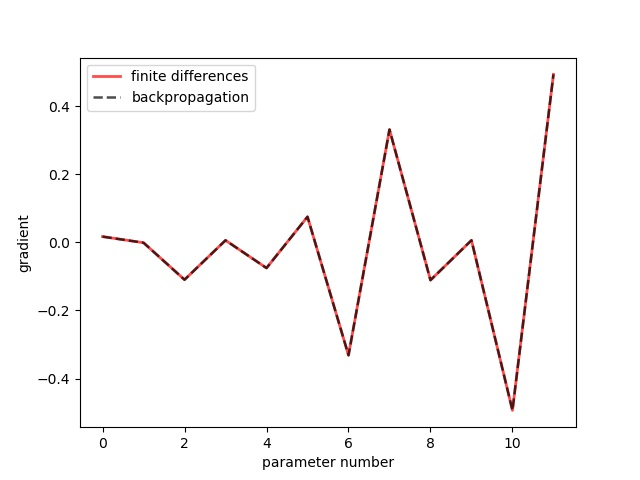
\includegraphics[width=0.8\textwidth]{gradient_differences_first-check_k1}
    \caption{Finite Differences vs Backprop Gradients with K=1, Loop Implementation, 2 Hidden Layer Neurons}
    \label{fig:gradient_differences_first-check_k1}
\end{figure}

And followed up with the same analysis using loops and a minibatch size of 10: \\

\begin{figure}[H]
    \centering
    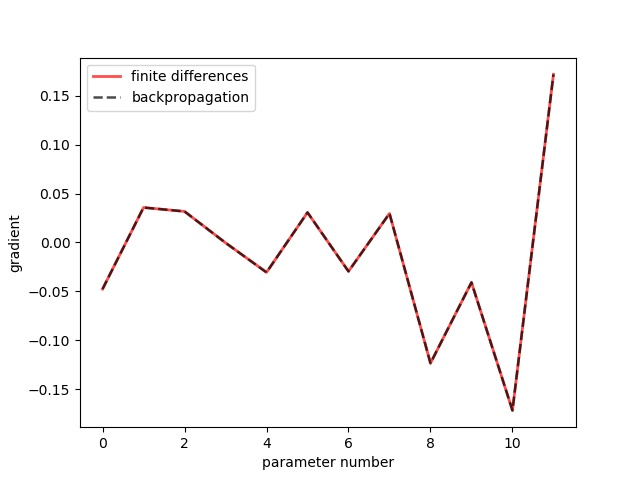
\includegraphics[width=0.8\textwidth]{gradient_differences_loop-added_k10}
    \caption{Finite Differences vs Backprop Gradients with K=10, Loop Implementation, 2 Hidden Layer Neurons}
    \label{fig:gradient_differences_loop-added_k10}
\end{figure}

We hope you agree that they both look good. \\

\subsection{Hyperparameter Choice and Decision Boundaries}

To evaluate the effect of the hyperparameters on our decision boundaries, we did a grid search over the following:

\begin{itemize}
    \item \textbf{Number of hidden units}: 5, 100
    \item \textbf{Learning rate}: $5 \times 10^{-2}$, $5 \times 10^{-3}$
    \item \textbf{L1 regularization lambda}: 0, 0.01
    \item \textbf{L2 regularization lambda}: 0, 0.01
    \item \textbf{Epochs}: 25, 100
\end{itemize}

We've attached all of the resulting images in a zip, and show only two here (one bad example, and one good example) for clarity. The number of hidden units has a large effect on capacity. All models trained with 5 hidden units were unable to learn a circular decision boundary: \\

\begin{figure}[H]
    \centering
    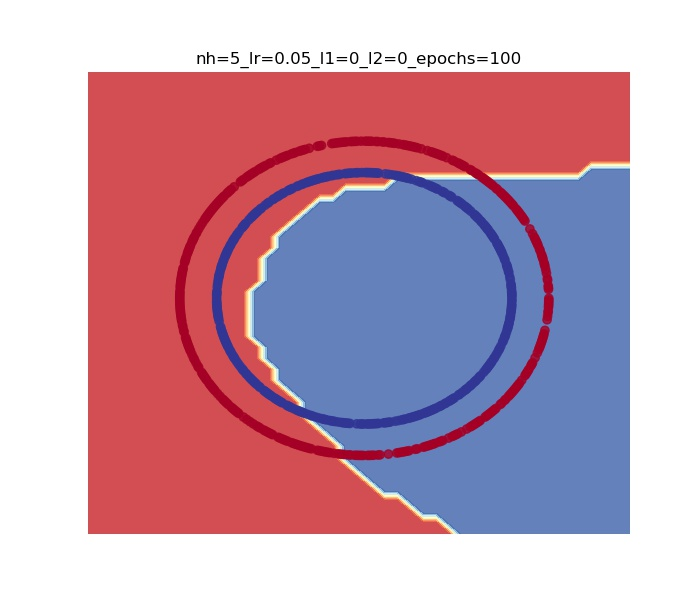
\includegraphics[width=0.8\textwidth]{decision_bad.jpg}
    \caption{Decision boundary with 5 hidden units.}
    \label{fig:decision_bad}
\end{figure}

We found that training the model for longer effectively increased it's capacity, as none of the 25 epoch models were able to perfectly learn the training set. Furthermore, larger values of regularization prevented the model from learning a perfect decision boundary. In some examples in the attached zip, you can see that too much regularization leads to poor gradients and no decision boundry at all. \\

\begin{figure}[H]
    \centering
    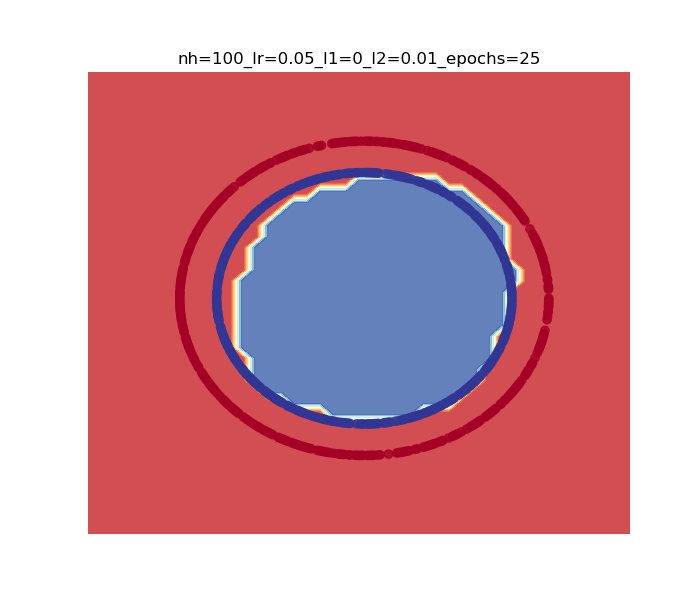
\includegraphics[width=0.8\textwidth]{decision_medium.jpg}
    \caption{Decision boundary with 100 hidden units and regularization.}
    \label{fig:decision_medium}
\end{figure}

A model trained for the full 100 epochs with no regularization and 100 hidden units was able to perfectly memorize the training data. \\

\begin{figure}[H]
    \centering
    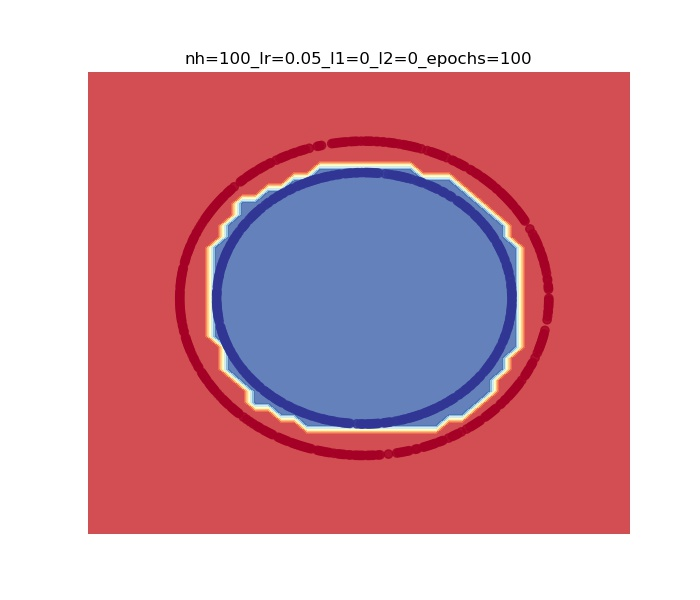
\includegraphics[width=0.8\textwidth]{decision_good.jpg}
    \caption{Decision boundary with 100 hidden units and no regularization.}
    \label{fig:decision_good}
\end{figure}

\subsection{Matrix Implementation}

See the previous \textbf{fprop} and \textbf{bprop} methods for the two implementations (loop and vector, see the if self.stupid\_loop statement). The key difference between the two methods is that the dimension of the input and output matricies have a singluar dimension, necessitating the use of resaping some vectors to act like matrices: (e.g.,  y = y.reshape(-1,1) # used for k=1 case). When this is done, all other matrix operations (dot products etc.) will work for all $k=n$, since the other matrix dimension will always batch the other parameters when doing dot products.\\

One key element is the averaging that happens at the end of the loop implementation. In the matrix version of backprop, there is an implicit sum of the gradients over the minibatch that happens right after the softmax, as part of a dot product. When using a loop, no such sum takes place. Therefore, the resulting vectors calculated (and stacked) in the vector implementation are averaged. In the matrix formulation, they are simply divided by the current batch size self.this\_k. \\

We then checked the gradients of this implementation with K=1 and K=10. \\

\begin{figure}[H]
    \centering
    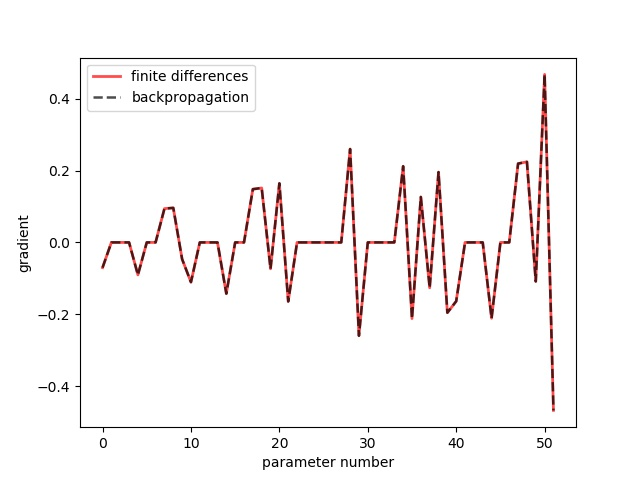
\includegraphics[width=0.8\textwidth]{gradient_differences_LOOP_k1}
    \caption{Finite Differences vs Backprop Gradients with K=1, Loop Implementation, 2 Hidden Layer Neurons}
    \label{fig:gradient_differences_LOOP_k1}
\end{figure}

\begin{figure}
    \centering
    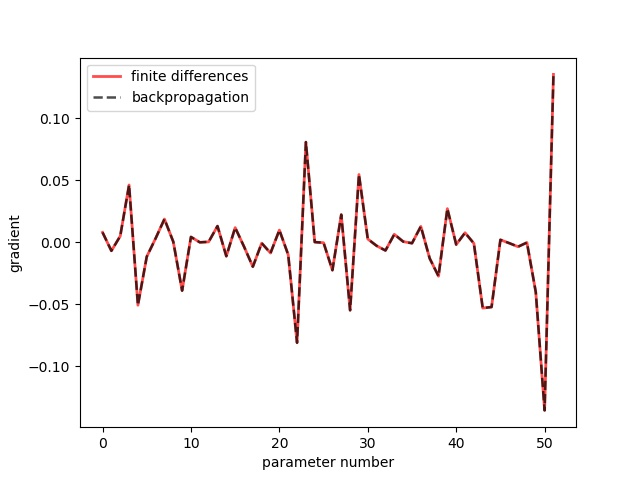
\includegraphics[width=0.8\textwidth]{gradient_differences_LOOP_k10}
    \caption{Finite Differences vs Backprop Gradients with K=10, Loop Implementation, 2 Hidden Layer Neurons}
    \label{fig:gradient_differences_LOOP_k10}
\end{figure}

\begin{figure}[H]
    \centering
    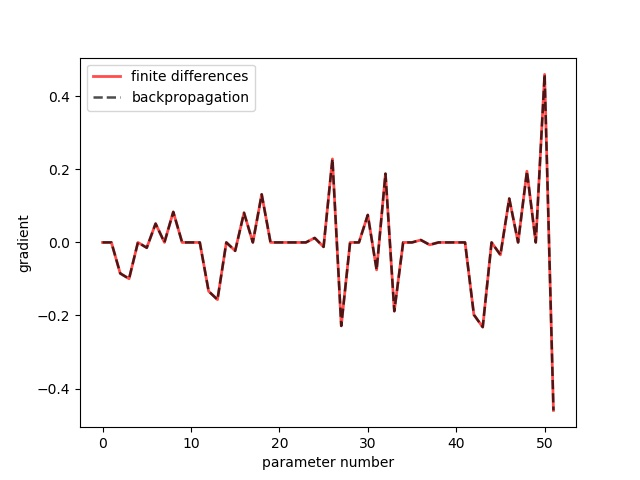
\includegraphics[width=0.8\textwidth]{gradient_differences_MATRIX_k1}
    \caption{Finite Differences vs Backprop Gradients with K=1, Matrix Implementation, 2 Hidden Layer Neurons}
    \label{fig:gradient_differences_MATRIX_k1}
\end{figure}

\begin{figure}[H]
    \centering
    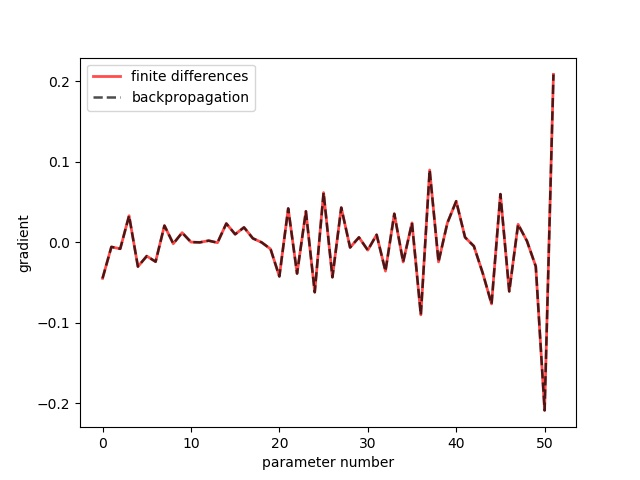
\includegraphics[width=0.8\textwidth]{gradient_differences_MATRIX_k10}
    \caption{Finite Differences vs Backprop Gradients with K=10, Matrix Implementation, 2 Hidden Layer Neurons}
    \label{fig:gradient_differences_MATRIX_k10}
\end{figure}

\subsection{Fashion MNIST}

The Loop implementation when run on minibatch of 100 for one epoch took approximately $10\times$ as long as the matrix implemntation: FASHION MNIST VECTOR time=218.50477123260498 vs LOOP time=2190.9738194942474 (see mlp\_log.txt, attached).

We trained a final model for 100 Epochs using the following hyperparameters:

\begin{itemize}
    \item k=256
    \item l1=0
    \item l2=0.001
    \item hidden units=50, 
    \item learning rate=0.001     
\end{itemize}

The following are the train, validation, and test loss / accuracy curves: \\

\begin{figure}[H]
    \centering
    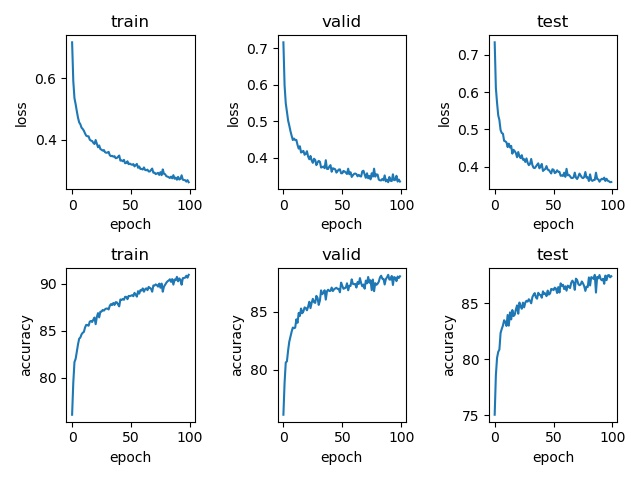
\includegraphics[width=0.8\textwidth]{curves}
    \caption{Train, Validation, and Test Learning Curves for Fashion MNIST, plotting Negative Log Liklihood and Accuracy}
    \label{fig:mnist_learning_curves}
\end{figure}

See the attached mlp\_log.txt for the full training log.

\end{document}